\chapter{Sperimentazione}

Gran parte del lavoro svolto nella fase di implementazione è stato fatto in stretta corrispondenza con lavori di sperimentazione, tramite tale processo è stato possibile infatti correggere errori, fissare nuovi obiettivi e implementare nuove funzionalità. 

Come obiettivo di sperimentazione è stato prefissato la realizzazione di un videogioco di combattimento tra carri con tecnologia digital twin.

\section{Integrazione di Arduino Alvik}
\begin{figure}[htb]
  \centering
  \includegraphics[width=1.0\textwidth, page=17]{Images/cristo.pdf}
  \caption{Architettura del gemello reale di Arduino Alvik.}
  \label{fig:rai-alvik}
\end{figure}
\subsubsection*{Real Agent Interface}
Come ampiamente trattato nel capitolo precedente, una concreta implementazione della classe \textit{BaseRAI} fornisce tutti gli strumenti necessari e di alto livello per fornire una interfaccia compatibile DTP, con la chicca di poter tipizzare le proprietà.

\begin{figure}[h!]
  \centering
  \includegraphics[width=0.7\textwidth, page=12]{Images/cristo.pdf}
  \caption{Interfaccia DTP del robot Arduino Alvik. }
  \label{fig:alvik-rai}
\end{figure}

Per il progetto di tesi è stata quindi realizzata una \textit{Real Agent Interface} per l'agente robotico mobile Arduino Alvik, completa di tutte le comodità necessarie al comando del sistema di locomozione dell'agente e il monitoraggio di stato, come velocità, posa, stato di carica della batteria. In \autoref{fig:alvik-rai} la interfaccia esposta API per mezzo di DTP.

\bigbreak
Tutti i sottosistemi dell'agente robotico, come locomozione, odometria, stato della batteria e sensori, sono esposti da una interfaccia API open source sviluppata da Arduino stessa \cite{arduino_alvik_repo}, pertanto consideriamo tale interfaccia una \textit{scatola nera} o \textit{black box} ai fini del lavoro svolto.

\bigbreak
Di seguito una descrizione delle proprietà e metodi esposti su DTP:

\begin{itemize}
	\item La proprietà \textbf{battery} indica lo stato di carica della batteria dell'agente, è un intero con valori da 0 a 100.
	\item La proprietà \textbf{is\_battery\_charging} indica se la batteria dell'agente è in ricarica, è di tipo booleano.
	\item La proprietà \textbf{pose} espone la posa del robot come array di 3 numeri \textit{float}, questi tre numeri devono essere interpretati come: un vettore a due dimensioni che rappresenta la posizione nel piano del robot in \textit{centimetri} di coordinate \textit{x} e \textit{y}; il terzo numero è un reale, con il nome in letteratura di \textit{theta}, rappresenta la direzione o angolo nel piano in \textit{radianti}.
	\item La proprietà \textbf{drive\_speed} espone un array di due numeri reali cui le singole componenti rappresentano rispettivamentee \textit{velocità lineare (cm/s)} e \textit{velocità angolare (rad/s)} dell'agente.
	\item Il metodo \textbf{drive} prende come parametri una \textit{velocità lineare (cm/s)} e una \textit{velocità angolare (rad/s)} obiettivo, l'agente allora proverà a muoversi a tali velocità: questa è l'unica funzione necessaria e sufficiente per la manipolazione spaziale del robot.
	\item Il metodo \textbf{reset\_pose} prende in input tre numeri reali \textit{x}, \textit{y} e \textit{theta} di tipo float che rappresentano una posa nello spazio, con lo scopo di ripristinare o sostituire la posa attuale con quella nuova. 
\end{itemize}

Non è necessaria una analisi approfondita di quanto esposto, poiché l'interfaccia espone direttamente funzionalità fornite dalle API di Arduino.

\subsubsection*{Gemello digitale}

Il \textbf{gemello digitale} invece, è dotato di modello tridimensionale dalla forma di un carro armato in stile cartonesco dotato di cingolati animati, forma e presenza fisica, ed emula un comportamento di movimento simile alla sua controparte reale.

Il suo model si muove per mezzo della funzione \textbf{drive}, analoga alla funzione del gemello reale, imposta velocità lineare e velocità angolare obiettivi all'interno dello stato dell'agente. Successivamente, durante l'elaborazione della fisica, il model proverà a muoversi nell'ambiente virtuale, in caso di collisioni con oggetti allora questo fermerà il suo moto lungo la specifica direzione e avrà allora velocità nulla.

Una volta calcolata la velocità finale, dopo l'elaborazione della fisica, viene estratto il vettore tridimensionale che ne rappresenta il moto, decomposto nuovamente in velocità lineare e angolare, e infine invocata una chiamata a procedura remota al corrispondente metodo \textit{drive} del gemello reale per mezzo di DTP, usando come parametri le velocità finali precedentemente calcolate.

Infine, la posa del model viene forzatamente posta in vicinanza al ghost usando interpolazione lineare.

\subsection*{Ulteriore software prodotto}
A supporto del lavoro svolto sul dispositivo embedded, sono state sviluppate una serie di utilità per semplificare la qualità di vita, comodamente disponibili all'interno di una interfaccia C++ e ordinate in rispettivi spazi dei nomi.
\subsubsection*{Funzione per la gestione dei LED}
La scheda a microcontrollore usata come piattaforma computazione dall'Arduino Alvik è un \textbf{Arduino ESP32 Nano BLE} dotato di tre LED, di cui due manipolabili tramite GPIO. Uno spazio dei nomi dedicato ai LED è stato prodotto, dotato di una procedura di inizializzazione \textit{init} e una serie di procedure per la manipolazione dei LED:
\begin{itemize}
	\item Un LED \textbf{RGB} manipolabile in logica di pulldown, sono state scritte funzioni per accendere o spegnere i tre colori \textbf{rosso}, \textbf{verde} e \textbf{blu} in modo non equivocabile.
	\item Un LED di colore arancione chiamato \textbf{builtin} in manipolabile in logica di pullup.
\end{itemize}
Tali funzionalità di aiuto sono state prodotte al fine di rendere non ambigua e pulita la manipolazione dei LED, indispensabili come mezzo visivo da parte dell'utente per la percezione dello stato del dispositivo.
\subsubsection*{Preferenze e stack di rete}
È stato sviluppando un sistema per la gestione e configurazione di credenziali della rete wireless e coordinate dell'host Godot ospitante l'ambiente virtuale e digital twin, così da non essere necessaria la scrittura di tali dati all'interno del sorgente e rendere più flessibile la riconfigurazione del dispositivo.

Tale sistema prevede la creazione di un task dedicato in ascolto sulla seriale del dispositivo, in attesa di una specifica payload JSON, una volta verificato che tale payload contiene la configurazione richiesta ( SSID, password, indirizzo e porta host ), la configurazione viene salvata nella memoria flash dell'ESP32 e quest'ultimo riavviato.

Sono state dedicate per il sistema di configurazione e stack di rete le funzioni: \verb|preferences::init| per inizializzare il sistema e creare il task in ascolto, \verb|preferences::get_preferences| per interrogare le preferenze, \verb|wifi::init| per inizializzare lo stack di rete e quindi la connessione alla rete wireless.

\section{Port di ENet per ESP32}
Il sistema operativo real-time \textit{FreeRTOS} per sistemi embedded non fornisce un classico ambiente di esecuzione come Windows e Linux, pertanto la libreria ENet non risulta direttamente compatibile con taile sistema.

Data l'importanza strategica di ENet ai fini del progetto, dopo una attenta analisi del sorgente e della documentazione di lwIP, lo stack di rete TCP/IP implementato in FreeRTOS, sono stati individuati una serie di parametri non compatibili usati nelle funzioni di manipolazione delle socket:
\begin{itemize}
	\item La funzione \textbf{getnameinfo} per la risoluzione del nome di rete di un indirizzo IP in lwIP non implementa il \textit{flag} \verb|NI_NAMEREQD|, tale flag obbliga la funzione a risolvere il nome di rete e in caso di fallimento restituire un errore, è stato sufficiente rimuovere l'uso di questo flag.
	\item Due funzioni, \textbf{recvmsg} e \textbf{sendmsg}, servono rispettivamente per accogliere e inviare messaggi tramite la socket, queste funzioni possono accettare il parametro di flag \verb|MSG_NOSIGNAL| in sistemi UNIX, tale parametro istruisce il sistema operativo di non inviare un segnale di arresto di tipo \verb|SIGPIPE| e quindi mandare in crash l'applicativo nel caso di \textit{disconnessione improvvisa della socket}, permettendo a quest'ultimo la gestione della condizione di errore. Il sistema operativo embedded usato dalla piattaforma ESP32, FreeRTOS, non implementa i segnali, è stato sufficiente ancora una volta rimuovere l'uso di questo flag in entrambe le invocazioni.
\end{itemize}

Da tale analisi e correzioni è stato prodotto un fork compatibile e liberamente disponibile \cite{enet_esp32}.
Si rassicura il lettore che le correzioni eseguite sono cautamente applicate se e solo se la piattaforma target di compilazione è un ESP32, usando le dovute direttive condizionali.

\section{Prove sperimentali}

\begin{figure}[htb]
  \centering
  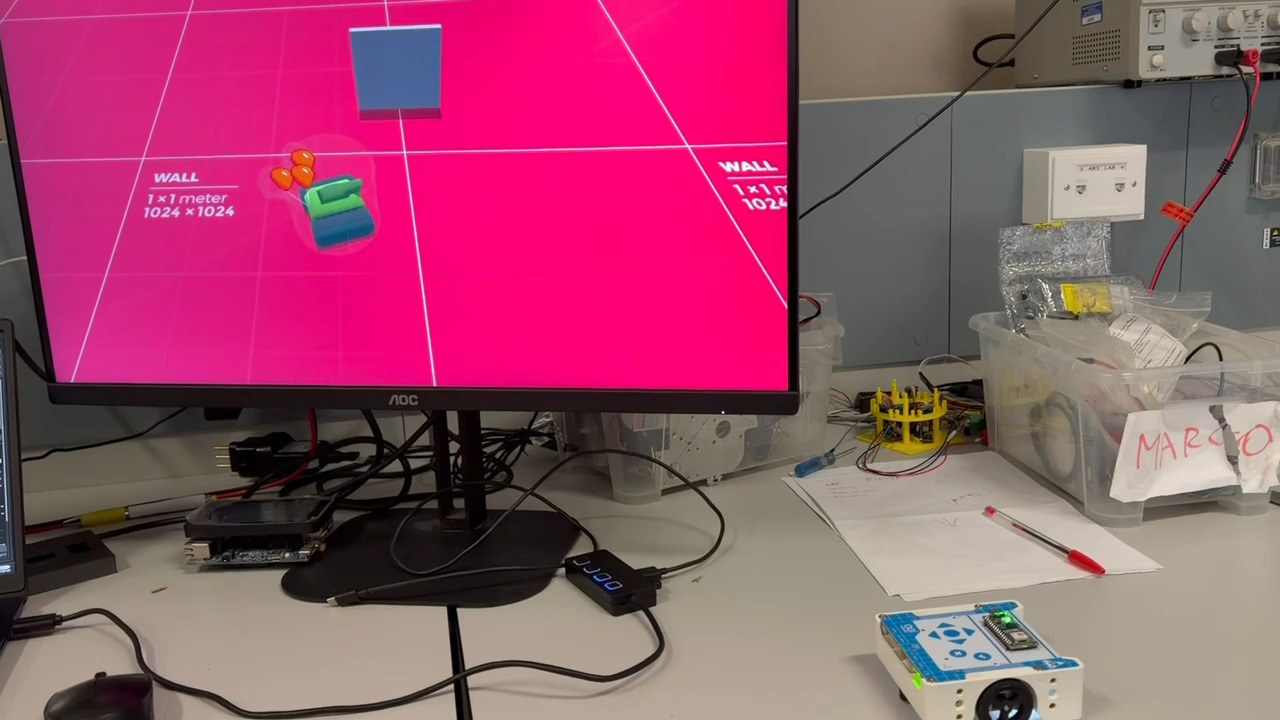
\includegraphics[width=1.0\textwidth]{Images/test-single.jpg}
  \caption{Gemello digitale singolo agente con guida a sterzata.}
  \label{fig:test-single}
\end{figure}
\subsection*{Singolo agente}
Le prime prove sperimentali hanno riguardato il controllo di un singolo gemello digitale. In questa fase l'autore ha costruito famigliarità con l'agente robotico e la cinematica differenziale; sono stati esplorati sistemi di controllo di guida differenti quali un \textit{controllo a sterzata} e un \textit{controllo polare} per la guida del robot. 

Infine, è stato costruito un ambiente virtuale per la navigazione, composto da un piano e un ostacolo, come mostrato in \autoref
{fig:test-single}. In tale ambiente è stato verificato che, qualora il gemello digitale collidesse con un muro e arrestasse il suo moto, di conseguenza anche il gemello reale arrestasse il suo moto.

\begin{figure}[htb]
  \centering
  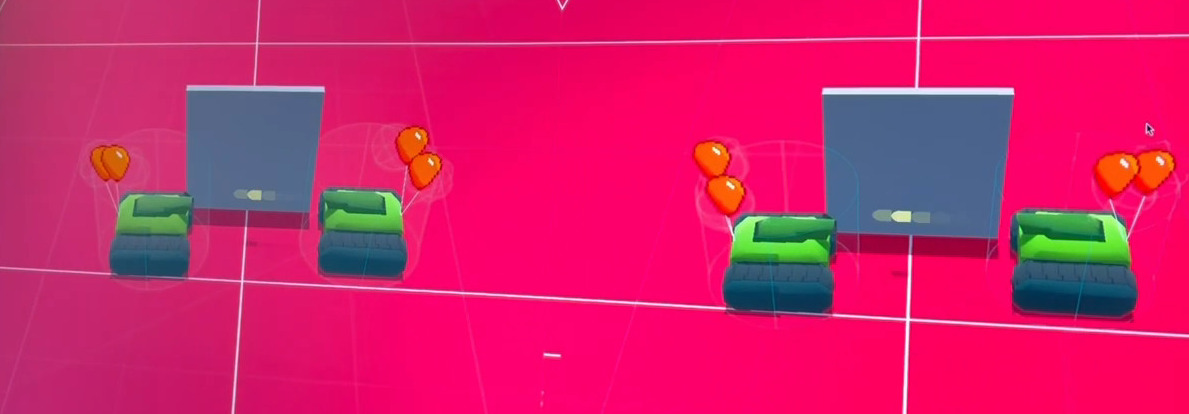
\includegraphics[width=1.0\textwidth]{Images/test-multi.jpg}
  \caption{Due istanze di Godot che espongono l'una all'altra un gemello digitale, implementati anche alcune feature di videogioco.}
  \label{fig:test-multi}
\end{figure}
\subsection*{Multi-agente distribuito}

Concluse le prove singolo-agente, è stata brevemente attestata la capacità del sistema software di gestire più agenti in una singola istanza.

Posto l'obiettivo di rendere distribuito il software, è stato svolto il lavoro necessario affiché sì potessero mettere in comunicazione più istanze di Godot in grado di esporre i gemelli digitali ad essa collegata: in tale fase sono state affrontate e superate con successo le eventuali complicazioni dovuta all'architettura della \textit{MultiplayerAPI}, in particolare la gestione della \textit{authority}, la istanziazione degli agenti remoti e la loro sincronizzazione.

In \autoref{fig:test-multi} sono mostrate due istanze separate di Godot che condividono ambiente virtuale e gemelli digitali.

\subsection*{Multi-agente distribuito e eterogeneo}
\begin{figure}[htb]
  \centering
  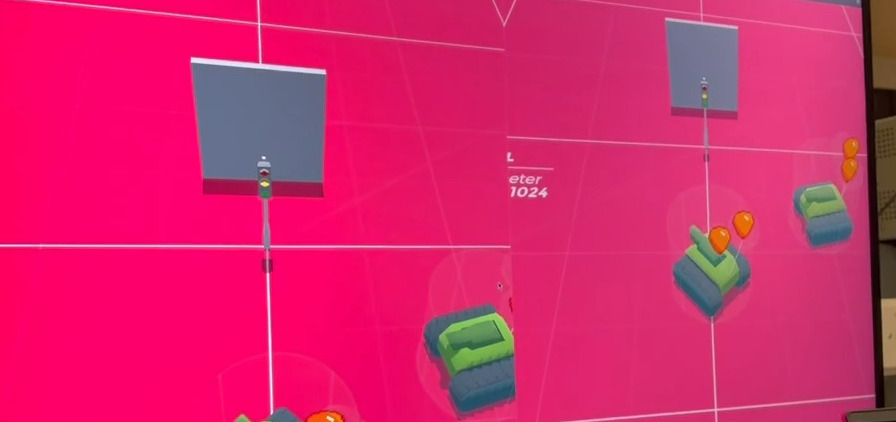
\includegraphics[width=1.0\textwidth]{Images/test-heterogeneous.jpg}
  \caption{Aggiunta di un terzo agente di tipo semaforo.}
  \label{fig:test-heterogeneous}
\end{figure}

Durante la stesura delle fasi conclusive dell'elaborato, è stato osservato che il progetto finale potesse arricchirsi ulteriormente permettendo il collegamento di tipi diversi di gemelli digitali.

Una volta implementata la logica all'interno del sistema, questa è stata corretta da eventuali errori e provata.

Come mostrato in Figura \ref{fig:test-heterogeneous}, è stato implementato un gemello digitale di un oggetto semaforo. Una relativa \textit{Real Agent Interface} è stata prodotta per tale oggetto ed eseguita da una board personalizzata dotata di microcontrollore Arduino Nano ESP32 BLE, il medesimo dell'Arduino Alvik, e di pulsantiera.

\subsection*{Realizzazione di un videogioco digital twin}
Come obiettivo conclusivo del percorso sperimentale, è stato prodotto un prototipo di videogioco di combattimento tra carri armati usando la tecnologia digital twin implementata.

Con l'obiettivo di supportare le dinamiche di gioco sulla infrastruttura realizzata, i gemelli digitali originali degli agenti Alvik sono stati estesi con le seguenti componenti e aggiunte:

\begin{itemize}
	\item È stato implementato un \textbf{sistema di vita} sul gemello digitale del carro. Ogni carro dispone di \textit{tre unità di vita}, raffigurate visivamente da altrettanti \textit{palloncini} legati al retro del carro. Ogni qualvolta il carro riceve un danno perde una unità di vita e un palloncino si scollega e vola via, inoltre: se il carro ha terminato le vite, il carro viene arrestato e viene mostrata visivamente una bandiera bianca a simboleggiarne la resa; altrimenti nel caso avesse ancora vite disponibili otterrà temporaneamente l'invincibilità e non potrà essere colpito da altri giocatori.
	\item A supporto del sistema precedente, è stato implementato un \textbf{sistema di shooting} dotato di tempo di ricarica. È stato prodotto un oggetto \textbf{bullet} (proiettile) e relativo assets, in grado di muoversi lungo un moto parabolico, collidere con oggetti e dotato di tempo di vita e massima distanza. Qualora in bullet interagisca con un carro avvierà le opportune routine di danno.
	\item Un sistema di ripristino è stato implementato affinché lo stato di vita dei carri possa essere ripristinato.
\end{itemize}

Al fine di rendere l'esperienza tanto più coinvolgente possibile, sono stati prodotti assets originali e personalizzati assets pubblici e gratuiti, inoltre è stata realizzata una opportuna arena di gioco.